\documentclass[utf8]{beamer}

%\usepackage[german]{babel}
\usepackage{ngerman}
\usepackage{xcolor}
\usepackage{graphicx}
\usepackage{tikz}

%Für den Header notwendig!
%\usepackage[percent]{overpic}

\usepackage{hyperref} % für korrekte Links

% Theme
\input{design_latex-template/beamerthemeFOSSAG.sty}


\title{Von Schlangen und Himbeerkuchen:\\Programmieren in der Welt von Minecraft}
\subtitle{Einführung}

\author{FOSS-AG}
\institute[FOSS AG]{\textbf{F}ree and \textbf{O}pen \textbf{S}ource \textbf{S}oftware \textbf{AG}}

\date{25/26. Okt 2017}

\begin{document}
	\begin{frame}
		\titlepage
	\end{frame}

	\begin{frame}{FOSS-AG - Wer, was und warum?}
		\begin{itemize}
			\item (Informatik-)Studierende
			\item Veranstaltungen zu Freier Software, Open Source und Linux
			\item Interesse wecken
			\item Informieren über die Relevanz von Freier Software im Alltag
		\end{itemize}
	\end{frame}
	
	\begin{frame}{Was ihr aus dem Workshop mitnehmt}
		\begin{itemize}
			\item Was ist ein Raspberry Pi
			\item Erste Erfahrungen mit einem Linux-Betriebssystem
			\item Programmieranfänge in Python
		\end{itemize}
	\end{frame}
	
	\begin{frame}{Was bedeutet freie Software?}
		\begin{itemize}
			\item Freie Benutzung einer Software
			\item Quellcode lesen und für die eigenen Bedürfnisse anpassen
			\item Freies Verteilen der Software, aber auch der eigenen Anpassungen
		\end{itemize}
	\end{frame}
	
	\begin{frame}{Linux - freie Software, freies Betriebssystem}
		Warum ist Linux cool?
		\begin{itemize}
			\item Open Source
			\item Gut zum Entwickeln
			\item Läuft auf den unterschiedlichsten Geräten
		\end{itemize}
	\end{frame}
	
	\begin{frame}{Raspberry Pi}
		\center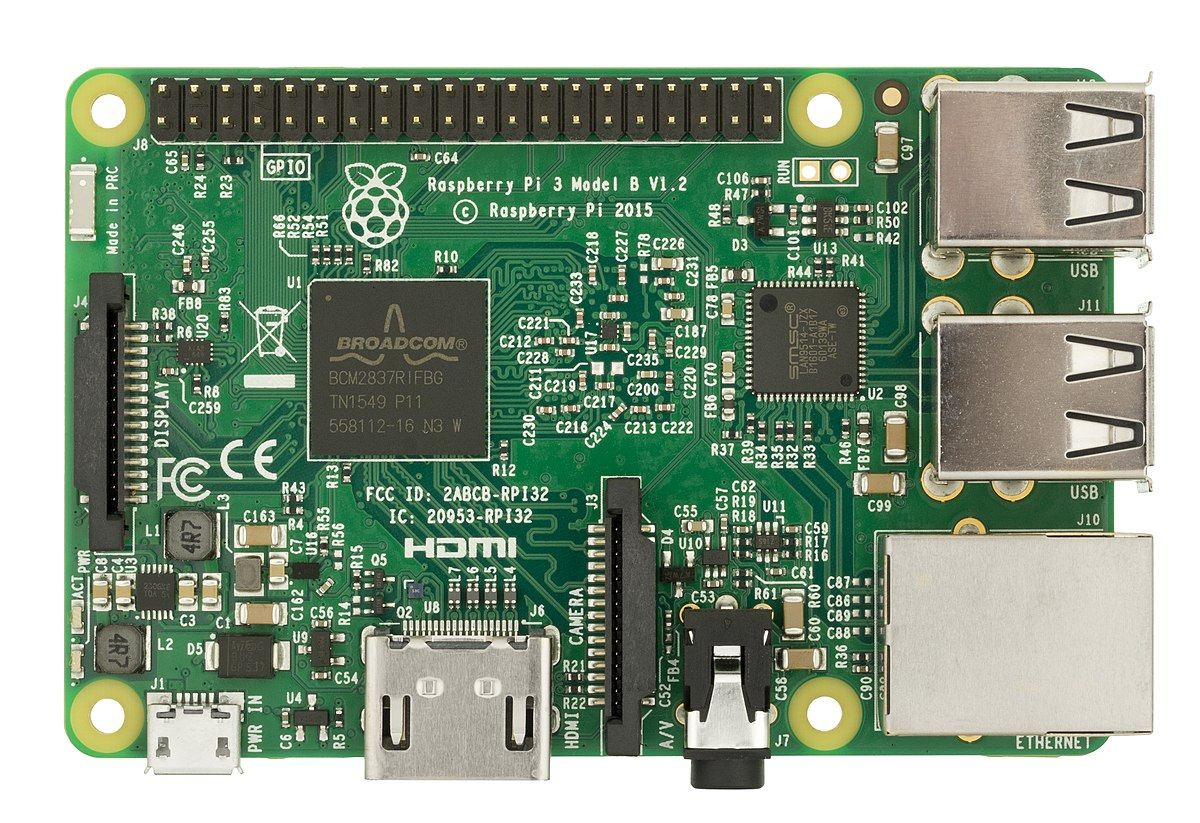
\includegraphics[width=\textwidth]{img/1200px-Raspberry-Pi-3-Flat-Top.jpg}
		
		%\tableofcontents[hideallsubsections]
	\end{frame}
	
	\begin{frame}{Vorteile des Raspberry Pi}
		
		\begin{itemize}
			\item Günstig
			\item Ungefährlich
			\item Relativ leistungsfähig
			\item Linux
			\item Quasi vollwertiger PC nur in klein
		\end{itemize}
	\end{frame}
	
	%\section{Die FOSS-AG}
	
	
	%\input{Einleitung.tex}
	
	%\section{Thema}
	%\input{blah.tex}
	
	
\end{document}